\chapter{Implementation}
\label{chapter:implementation}

% Arkkitehtuuri
% Työvoita
% Teknologia
% EI ohjelmadokumentti!

Here we describe how the methods are implemented to achieve the 
clustering. First we describe how the raw text data is 
pre-processed 

We implemented the workflow for clustering using Python's 
\texttt{scikit-learn} package completed with 
pre-processing managed with \texttt{doit} workflow. See Figure 
\ref{fig:wf} for the workflow graph.

\begin{figure}[ht]
  \begin{center}    
    % Graphic for TeX using PGF
% Title: /home/jlehtonen/nextcloud/synkronoitu/dippa/clustering/doc/images/workflow.dia
% Creator: Dia v0.97.3
% CreationDate: Mon Dec  9 05:57:48 2019
% For: jlehtonen
% \usepackage{tikz}
% The following commands are not supported in PSTricks at present
% We define them conditionally, so when they are implemented,
% this pgf file will use them.
\ifx\du\undefined
  \newlength{\du}
\fi
\setlength{\du}{15\unitlength}
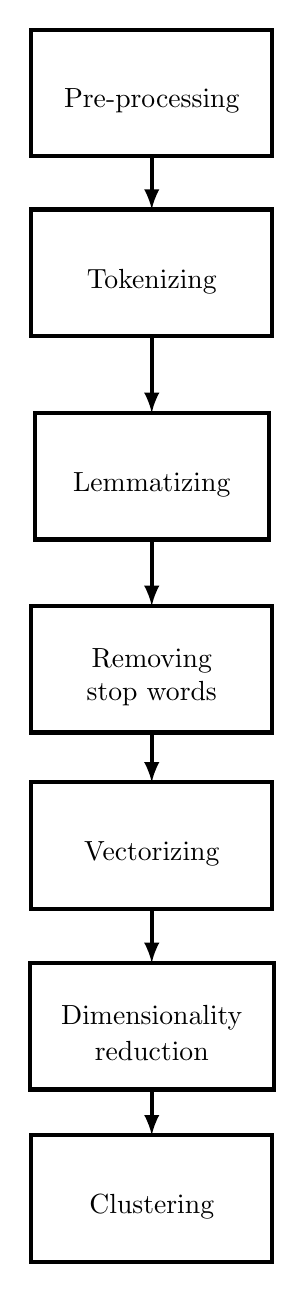
\begin{tikzpicture}
\pgftransformxscale{1.000000}
\pgftransformyscale{-1.000000}
\definecolor{dialinecolor}{rgb}{0.000000, 0.000000, 0.000000}
\pgfsetstrokecolor{dialinecolor}
\definecolor{dialinecolor}{rgb}{1.000000, 1.000000, 1.000000}
\pgfsetfillcolor{dialinecolor}
\definecolor{dialinecolor}{rgb}{1.000000, 1.000000, 1.000000}
\pgfsetfillcolor{dialinecolor}
\fill (5.932500\du,3.900000\du)--(5.932500\du,6.950000\du)--(11.730000\du,6.950000\du)--(11.730000\du,3.900000\du)--cycle;
\pgfsetlinewidth{0.100000\du}
\pgfsetdash{}{0pt}
\pgfsetdash{}{0pt}
\pgfsetmiterjoin
\definecolor{dialinecolor}{rgb}{0.000000, 0.000000, 0.000000}
\pgfsetstrokecolor{dialinecolor}
\draw (5.932500\du,3.900000\du)--(5.932500\du,6.950000\du)--(11.730000\du,6.950000\du)--(11.730000\du,3.900000\du)--cycle;
% setfont left to latex
\definecolor{dialinecolor}{rgb}{0.000000, 0.000000, 0.000000}
\pgfsetstrokecolor{dialinecolor}
\node at (8.831250\du,5.620000\du){Pre-processing};
% setfont left to latex
\definecolor{dialinecolor}{rgb}{0.000000, 0.000000, 0.000000}
\pgfsetstrokecolor{dialinecolor}
\node[anchor=west] at (8.831250\du,5.425000\du){};
\definecolor{dialinecolor}{rgb}{1.000000, 1.000000, 1.000000}
\pgfsetfillcolor{dialinecolor}
\fill (5.932500\du,8.230000\du)--(5.932500\du,11.280000\du)--(11.730000\du,11.280000\du)--(11.730000\du,8.230000\du)--cycle;
\pgfsetlinewidth{0.100000\du}
\pgfsetdash{}{0pt}
\pgfsetdash{}{0pt}
\pgfsetmiterjoin
\definecolor{dialinecolor}{rgb}{0.000000, 0.000000, 0.000000}
\pgfsetstrokecolor{dialinecolor}
\draw (5.932500\du,8.230000\du)--(5.932500\du,11.280000\du)--(11.730000\du,11.280000\du)--(11.730000\du,8.230000\du)--cycle;
% setfont left to latex
\definecolor{dialinecolor}{rgb}{0.000000, 0.000000, 0.000000}
\pgfsetstrokecolor{dialinecolor}
\node at (8.831250\du,9.950000\du){};
% setfont left to latex
\definecolor{dialinecolor}{rgb}{0.000000, 0.000000, 0.000000}
\pgfsetstrokecolor{dialinecolor}
\node at (8.831250\du,9.976250\du){Tokenizing};
% setfont left to latex
\definecolor{dialinecolor}{rgb}{0.000000, 0.000000, 0.000000}
\pgfsetstrokecolor{dialinecolor}
\node[anchor=west] at (8.840594\du,17.305000\du){};
\definecolor{dialinecolor}{rgb}{1.000000, 1.000000, 1.000000}
\pgfsetfillcolor{dialinecolor}
\fill (6.014375\du,13.130000\du)--(6.014375\du,16.180000\du)--(11.648125\du,16.180000\du)--(11.648125\du,13.130000\du)--cycle;
\pgfsetlinewidth{0.100000\du}
\pgfsetdash{}{0pt}
\pgfsetdash{}{0pt}
\pgfsetmiterjoin
\definecolor{dialinecolor}{rgb}{0.000000, 0.000000, 0.000000}
\pgfsetstrokecolor{dialinecolor}
\draw (6.014375\du,13.130000\du)--(6.014375\du,16.180000\du)--(11.648125\du,16.180000\du)--(11.648125\du,13.130000\du)--cycle;
% setfont left to latex
\definecolor{dialinecolor}{rgb}{0.000000, 0.000000, 0.000000}
\pgfsetstrokecolor{dialinecolor}
\node at (8.831250\du,14.850000\du){Lemmatizing};
\definecolor{dialinecolor}{rgb}{1.000000, 1.000000, 1.000000}
\pgfsetfillcolor{dialinecolor}
\fill (5.932500\du,17.780000\du)--(5.932500\du,20.830000\du)--(11.730000\du,20.830000\du)--(11.730000\du,17.780000\du)--cycle;
\pgfsetlinewidth{0.100000\du}
\pgfsetdash{}{0pt}
\pgfsetdash{}{0pt}
\pgfsetmiterjoin
\definecolor{dialinecolor}{rgb}{0.000000, 0.000000, 0.000000}
\pgfsetstrokecolor{dialinecolor}
\draw (5.932500\du,17.780000\du)--(5.932500\du,20.830000\du)--(11.730000\du,20.830000\du)--(11.730000\du,17.780000\du)--cycle;
% setfont left to latex
\definecolor{dialinecolor}{rgb}{0.000000, 0.000000, 0.000000}
\pgfsetstrokecolor{dialinecolor}
\node at (8.831250\du,19.100000\du){Removing};
% setfont left to latex
\definecolor{dialinecolor}{rgb}{0.000000, 0.000000, 0.000000}
\pgfsetstrokecolor{dialinecolor}
\node at (8.831250\du,19.900000\du){stop words};
\definecolor{dialinecolor}{rgb}{1.000000, 1.000000, 1.000000}
\pgfsetfillcolor{dialinecolor}
\fill (5.932500\du,22.030000\du)--(5.932500\du,25.080000\du)--(11.730000\du,25.080000\du)--(11.730000\du,22.030000\du)--cycle;
\pgfsetlinewidth{0.100000\du}
\pgfsetdash{}{0pt}
\pgfsetdash{}{0pt}
\pgfsetmiterjoin
\definecolor{dialinecolor}{rgb}{0.000000, 0.000000, 0.000000}
\pgfsetstrokecolor{dialinecolor}
\draw (5.932500\du,22.030000\du)--(5.932500\du,25.080000\du)--(11.730000\du,25.080000\du)--(11.730000\du,22.030000\du)--cycle;
% setfont left to latex
\definecolor{dialinecolor}{rgb}{0.000000, 0.000000, 0.000000}
\pgfsetstrokecolor{dialinecolor}
\node at (8.831250\du,23.750000\du){Vectorizing};
\definecolor{dialinecolor}{rgb}{1.000000, 1.000000, 1.000000}
\pgfsetfillcolor{dialinecolor}
\fill (5.892500\du,26.380000\du)--(5.892500\du,29.430000\du)--(11.770000\du,29.430000\du)--(11.770000\du,26.380000\du)--cycle;
\pgfsetlinewidth{0.100000\du}
\pgfsetdash{}{0pt}
\pgfsetdash{}{0pt}
\pgfsetmiterjoin
\definecolor{dialinecolor}{rgb}{0.000000, 0.000000, 0.000000}
\pgfsetstrokecolor{dialinecolor}
\draw (5.892500\du,26.380000\du)--(5.892500\du,29.430000\du)--(11.770000\du,29.430000\du)--(11.770000\du,26.380000\du)--cycle;
% setfont left to latex
\definecolor{dialinecolor}{rgb}{0.000000, 0.000000, 0.000000}
\pgfsetstrokecolor{dialinecolor}
\node at (8.831250\du,27.700000\du){Dimensionality};
% setfont left to latex
\definecolor{dialinecolor}{rgb}{0.000000, 0.000000, 0.000000}
\pgfsetstrokecolor{dialinecolor}
\node at (8.831250\du,28.500000\du){reduction};
\pgfsetlinewidth{0.100000\du}
\pgfsetdash{}{0pt}
\pgfsetdash{}{0pt}
\pgfsetbuttcap
{
\definecolor{dialinecolor}{rgb}{0.000000, 0.000000, 0.000000}
\pgfsetfillcolor{dialinecolor}
% was here!!!
\pgfsetarrowsend{latex}
\definecolor{dialinecolor}{rgb}{0.000000, 0.000000, 0.000000}
\pgfsetstrokecolor{dialinecolor}
\draw (8.831250\du,6.950000\du)--(8.831250\du,8.230000\du);
}
\pgfsetlinewidth{0.100000\du}
\pgfsetdash{}{0pt}
\pgfsetdash{}{0pt}
\pgfsetbuttcap
{
\definecolor{dialinecolor}{rgb}{0.000000, 0.000000, 0.000000}
\pgfsetfillcolor{dialinecolor}
% was here!!!
\pgfsetarrowsend{latex}
\definecolor{dialinecolor}{rgb}{0.000000, 0.000000, 0.000000}
\pgfsetstrokecolor{dialinecolor}
\draw (8.831250\du,11.280000\du)--(8.831250\du,13.130000\du);
}
\pgfsetlinewidth{0.100000\du}
\pgfsetdash{}{0pt}
\pgfsetdash{}{0pt}
\pgfsetbuttcap
{
\definecolor{dialinecolor}{rgb}{0.000000, 0.000000, 0.000000}
\pgfsetfillcolor{dialinecolor}
% was here!!!
\pgfsetarrowsend{latex}
\definecolor{dialinecolor}{rgb}{0.000000, 0.000000, 0.000000}
\pgfsetstrokecolor{dialinecolor}
\draw (8.831250\du,16.180000\du)--(8.831250\du,17.780000\du);
}
\pgfsetlinewidth{0.100000\du}
\pgfsetdash{}{0pt}
\pgfsetdash{}{0pt}
\pgfsetbuttcap
{
\definecolor{dialinecolor}{rgb}{0.000000, 0.000000, 0.000000}
\pgfsetfillcolor{dialinecolor}
% was here!!!
\pgfsetarrowsend{latex}
\definecolor{dialinecolor}{rgb}{0.000000, 0.000000, 0.000000}
\pgfsetstrokecolor{dialinecolor}
\draw (8.831250\du,20.830000\du)--(8.831250\du,22.030000\du);
}
% setfont left to latex
\definecolor{dialinecolor}{rgb}{0.000000, 0.000000, 0.000000}
\pgfsetstrokecolor{dialinecolor}
\node[anchor=west] at (8.831250\du,27.905000\du){};
% setfont left to latex
\definecolor{dialinecolor}{rgb}{0.000000, 0.000000, 0.000000}
\pgfsetstrokecolor{dialinecolor}
\node[anchor=west] at (8.831250\du,27.905000\du){};
\definecolor{dialinecolor}{rgb}{1.000000, 1.000000, 1.000000}
\pgfsetfillcolor{dialinecolor}
\fill (5.932500\du,30.530000\du)--(5.932500\du,33.580000\du)--(11.730000\du,33.580000\du)--(11.730000\du,30.530000\du)--cycle;
\pgfsetlinewidth{0.100000\du}
\pgfsetdash{}{0pt}
\pgfsetdash{}{0pt}
\pgfsetmiterjoin
\definecolor{dialinecolor}{rgb}{0.000000, 0.000000, 0.000000}
\pgfsetstrokecolor{dialinecolor}
\draw (5.932500\du,30.530000\du)--(5.932500\du,33.580000\du)--(11.730000\du,33.580000\du)--(11.730000\du,30.530000\du)--cycle;
% setfont left to latex
\definecolor{dialinecolor}{rgb}{0.000000, 0.000000, 0.000000}
\pgfsetstrokecolor{dialinecolor}
\node at (8.831250\du,32.250000\du){Clustering};
% setfont left to latex
\definecolor{dialinecolor}{rgb}{0.000000, 0.000000, 0.000000}
\pgfsetstrokecolor{dialinecolor}
\node[anchor=west] at (8.831250\du,32.055000\du){};
\pgfsetlinewidth{0.100000\du}
\pgfsetdash{}{0pt}
\pgfsetdash{}{0pt}
\pgfsetbuttcap
{
\definecolor{dialinecolor}{rgb}{0.000000, 0.000000, 0.000000}
\pgfsetfillcolor{dialinecolor}
% was here!!!
\pgfsetarrowsend{latex}
\definecolor{dialinecolor}{rgb}{0.000000, 0.000000, 0.000000}
\pgfsetstrokecolor{dialinecolor}
\draw (8.831250\du,25.080000\du)--(8.831250\du,26.380000\du);
}
\pgfsetlinewidth{0.100000\du}
\pgfsetdash{}{0pt}
\pgfsetdash{}{0pt}
\pgfsetbuttcap
{
\definecolor{dialinecolor}{rgb}{0.000000, 0.000000, 0.000000}
\pgfsetfillcolor{dialinecolor}
% was here!!!
\pgfsetarrowsend{latex}
\definecolor{dialinecolor}{rgb}{0.000000, 0.000000, 0.000000}
\pgfsetstrokecolor{dialinecolor}
\draw (8.831250\du,29.430000\du)--(8.831250\du,30.530000\du);
}
\end{tikzpicture}

    \caption{The workflow of the clustering.}
    \label{fig:wf}
  \end{center}
\end{figure}

\section{Prepocessing}
First data was read from raw files obtained from publishers. 
%(Actually YL probably also preprocessed data before passing it 
% to me.)
Unrelevant metadata fields like \emph{journal}, \emph{year}, 
\emph{issn} and \emph{references} were omitted and the relevant 
were read into a dictionary. We choose to keep \emph{title}, 
\emph{abstract} and \emph{keyword} fields. Terms in keyword 
fields were concatenated into combined 
terms: ``allergic\_contact\_dermatitis''. This is related 
to the counting of words in a metadata and will be explained 
soon.

\section{Tokenizing}
The metadata in chosen fields was then tokenized with
punctuation and whitespace separating the tokens (words). We 
get for example ``Pluto is a smart dog'' --> ``Pluto'', ``is'', 
``a'', ``smart'' and ``dog''. This strategy is known as \emph{Bag 
of Words} representation because each word is taken as is 
ignoring all its positional information in relation to other 
words. Another option would be to form n-grams to preserve the 
meaning of combined terms. Eg. ``allergic'', ``contact'', 
``dermatitis'', ``allergic contact'', ``contact dermatitis''. Here 
single words are called 1-grams, word pairs are called 2-grams and 
so on. Counting the n-grams would expand the feature space n-fold 
though and we wanted to avoid the computational cost.

\section{Lemmatizing}
After getting the words we lemmatized them against WordNet 
lemmatizer.
% After parsing data is written to interim files.
We choose to remove all plain numbers from
data. Another option is to replace numbers with dummy '\#NUMBER'.
That could help separate natural sciences from humanities. Because 
we didn't have proper knowledge on the issue removal was chosen. So 
numbers would be ignored. That would be a more neutral way to treat 
them. \fixme{How? Explain...}

\section{Removing stop words}
Stop words had to be lemmatized also before data could be 
filtered to remove those. We used NLTK modules English stop words 
combined with \texttt{scikit-learn's} stop words and our own stop 
word list consisting mainly standard publisher notices 
(\emph{``reserved'', ``rights''} and publising years).

\section{Counting}
After removing stop words term frequencies were counted and 
normalized with inverse document frequencies (\emph{tf-idf} 
normalization). In this point we ahve the data vectorized.

\section{Clustering}
Running preliminary tests for 2000 publications with tf-idf's maximum and 
minimum document frequencies set to $max_df=0.5$ 
and $min_df=2$ (integers denote absolute count value) respectively
resulted a feature space of 3372 terms and a stop word list of 7475 
terms. The stop word list included 352 a priori set words and words
that occurred in too many ($max_df$) or too few ($min_df$) 
documents. Terms that were filtered out as too frequent or too few
were for example: ``haemoglobin\_a'', ``jacobian\_matrix'', 
``parthenogenetic'', ``chelation\_by\_saccharide\_molecules'', 
``leg\_blood\_supply'', ``computational\_fluid\_dynamics'', 
``pigment'', ``hdtv'', ``nicotinic\_receptor''.

(Interesting would be to know the frequencies of the filtered-out 
terms. It didn't come out straight from TfIdfVectroizer class used 
but taking different levels of $min_df$ and $max_df$ could be used 
to view different frequency groups.)

When trying with $max_df=0.6$ we get feature space of XXXX and 
YYYY stop words.

